\documentclass[12pt,letterpaper]{hmcpset}
\usepackage[margin=1in]{geometry}
\usepackage{graphicx}

% info for header block in upper right hand corner
\name{ }
\class{Math 60}
\assignment{HW 7}
\duedate{Wednesday, May 25, 2016}

\newcommand{\pn}[1]{\left( #1 \right)}
\newcommand{\abs}[1]{\left| #1 \right|}
\newcommand{\bk}[1]{\left[ #1 \right]}

\newcommand{\RR}{\mathbb{R}}

\renewcommand{\labelenumi}{{(\alph{enumi})}}

\begin{document}

\problemlist{4.2.\{28, 30, 34, 46\}, 4.3.\{6, 24, 26\}}

\begin{problem}[Colley 4.2.28]
    Show that the largest rectangular box having a fixed surface area
    must be a cube.
\end{problem}
\begin{solution}
    \vfill
\end{solution}
\newpage

\begin{problem}[Colley 4.2.30]
    Find the points on the surface $xy+z^2=4$ that are closest to the
    origin. Be sure to give a convincing argument that your answer is
    correct.
\end{problem}
\begin{solution}
    \vfill
\end{solution}
\newpage

\begin{problem}[Colley 4.2.34]
    A metal plate has the shape of the region $x^2+y^2\leq 1$. The
    plate is heated so that the temperature at any point $(x,y)$ on it
    is indicated by
    \[
        T(x,y)=2x^2+y^2-y+3.
    \]
    Find the hottest and coldest points on the plate and the
    temperature at each of these points. (Hint: Parameterize the
    boundary of the plate in order to find any critical points there.)
\end{problem}
\begin{solution}
    \vfill
\end{solution}
\newpage

\begin{problem}[Colley 4.2.46]
    In Exercises 46-48, (a) find all critical points of the given
    function $f$ and identify their nature as local extrema and (b)
    determine, with explanation, any global extrema of $f$.
    \[
        f(x,y)=e^{x^2+5y^2}
    \]
\end{problem}
\begin{solution}
    \vfill
\end{solution}
\newpage

\begin{problem}[Colley 4.3.6]
    In Exercises 2-12, use Lagrange multipliers to identify the
    critical points of $f$ subject to the given constraints.
    \[
        f(x,y,z)=x^2+y^2+z^2,\quad x+y-z=1
    \]
\end{problem}
\begin{solution}
    \vfill
\end{solution}
\newpage

\begin{problem}[Colley 4.3.24]
    You are sending a birthday present to your calculus
    instructor. Fly-By-Night Delivery Service insists that any package
    it ships be such that the sum of the length plus the girth be at
    most 108 in. (The girth is the perimeter of the cross section
    perpendicular to the length axis---see Figure 4.31.) What are the
    dimensions of the largest present you can send?
    \begin{center}
        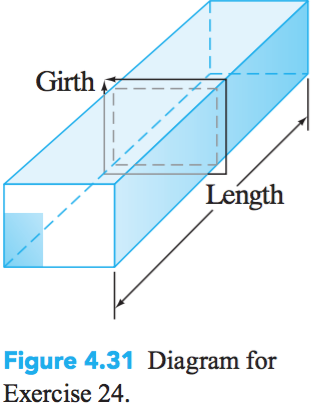
\includegraphics[scale=0.8]{img/4_3_24}
    \end{center}
\end{problem}
\begin{solution}
    \vfill
\end{solution}
\newpage

\begin{problem}[Colley 4.3.26]
    An industrious farmer is designing a silo to hold her $900\pi$
    ft$^3$ supply of grain. The silo is to be cylindrical in shape with
    a hemispherical roof. (See Figure 4.32.) Suppose that it costs
    five times as much (per square foot of sheet metal used) to
    fashion the roof of the silo as it does to make the circular floor
    and twice as much to make the cylindrical walls as the floor. If
    you were to act as consultant for this project, what dimensions
    would you recommend so that the \textit{total} cost would be a
    minimum? On what do you base your recommendation? (Assume that the
    entire silo can be filled with grain.)
    \begin{center}
        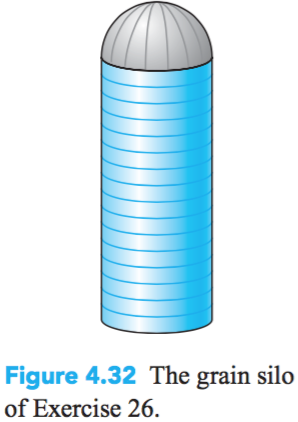
\includegraphics[scale=0.8]{img/4_3_26}
    \end{center}
\end{problem}
\begin{solution}
    \vfill
\end{solution}
\end{document}
